%===============================================================================
%===============================================================================
%
\clearpage
%
\subsection{Example-0204-u \texttt{[PLAUSIBLE]}}
%
Example uses user-defined hexahedral mesh (tibialis anterior with skin)
in CHeart mesh format and solves a static problem,
i.e., applies the boundary conditions in one step.\\[3ex]

%===============================================================================
%
\subsubsection{Mathematical model - 3D}
%
We solve the following scalar equation,
%
\begin{align}
    \nabla \cdot \boldsymbol{P} (\boldsymbol{u}, t) = \boldsymbol{0} & &&\Omega,
\end{align}
%
with 1st Piola-Kirchhoff stress tensor in $d$ dimensions,
%
\begin{align}
    \boldsymbol{P} &= \frac{2 \mu}{[\det F]^{2/d}} \left( \boldsymbol{F} - \frac{\boldsymbol{F} : \boldsymbol{F}}{d} \boldsymbol{F}^{-T} \right) + p \boldsymbol{F}^{-T}
\end{align}
%
corresponding to a Neo-Hookean constitutive law (Neo-Hooke parameter $\mu$)
with Dirichlet boundary conditions
%
\begin{align}
    u_x = u_y = u_z = 0 & && \text{BOTTOM}, \\
		u_x = u_y = u_z = 2 & && \text{TOP}.
\end{align}
%
Undeformed geometry and deformed geometry with pressure field
in Figure~\ref{example-0204-u-iron-reference-undeformed-geometry-deformed-geometry-pressure-fig} (left).
Deformed geometry with displacement field
in Figure~\ref{example-0204-u-iron-reference-deformed-geometry-displacement-fig}.

Note: The pressure has an opposite sign compared to CHeart and KerMOR.
%
%===============================================================================
%
\subsubsection{Computational model}
%
\begin{itemize}
    \item{Commandline arguments are:}
        \subitem{string: Mesh input file}
        \subitem{integer: solver type (0 - iterative, 1 - direct)}
        \subitem{integer: Jacobian type (0 - analytic, 1 - finite difference)}
        \subitem{float: 1st Mooney-Rivlin parameter}
        \subitem{float: 2nd Mooney-Rivlin parameter (set to zero)}
        \subitem{float: absolute displacement at top surface in each coordinate direction}
        \subitem{integer: number of load increments}
        \subitem{integer: BC type at top surface(0 - Dirichlet BC, 1 - Neumann\_integrated, 2 - Neumann\_point)}
    \item{Commandline arguments for tests are:}
        \subitem{TBD}
    \item{Note: Binary uses command line arguments to search for the relevant mesh files if user-defined meshes are selected.}
\end{itemize}
%
%===============================================================================
%
\subsubsection{Result summary}
%
We use CHeart revision 6411 to compare all displacement components and the
pressure field (reference value: RSE of normalized RMSE of components is
$0.00484848482722$).

We also compare against an OpenCMISS-iron reference run.
%
\verbatiminput{examples/example-0204-u/results/results.summary}
\verbatiminput{examples/example-0204-u/results/failed.tests}
%
\begin{figure}[h!]
    \centering
    \includegraphics[width=0.49\columnwidth]{examples/example-0204-u/doc/figures/undeformed_geometry.eps}
    \includegraphics[width=0.49\columnwidth]{examples/example-0204-u/doc/figures/deformed_geometry-pressure.eps}
    \caption{Iron reference run, undeformed geometry and deformed geometry with pressure field.}
    \label{example-0204-u-iron-reference-undeformed-geometry-deformed-geometry-pressure-fig}
\end{figure}
%
\begin{figure}[h!]
    \centering
    \includegraphics[width=0.49\columnwidth]{examples/example-0204-u/doc/figures/deformed_geometry-displacementM.eps}
    \includegraphics[width=0.49\columnwidth]{examples/example-0204-u/doc/figures/deformed_geometry-displacementX.eps}
    \includegraphics[width=0.49\columnwidth]{examples/example-0204-u/doc/figures/deformed_geometry-displacementY.eps}
    \includegraphics[width=0.49\columnwidth]{examples/example-0204-u/doc/figures/deformed_geometry-displacementZ.eps}
    \caption{Iron reference run, top-left to bottom-right: Deformed geometry with displacement field magnitude, x-component, y-component and z-component.}
    \label{example-0204-u-iron-reference-deformed-geometry-displacement-fig}
\end{figure}
%
\begin{figure}[h!]
    \centering
    \includegraphics[width=0.49\linewidth]{examples/example-0204-u/doc/figures/cheart_pressure_timestep_0000000001.png}~\\
    \includegraphics[width=0.49\linewidth]{examples/example-0204-u/doc/figures/cheart_displacementm_timestep_0000000001.png}
    \includegraphics[width=0.49\linewidth]{examples/example-0204-u/doc/figures/cheart_displacementx_timestep_0000000001.png}
    \includegraphics[width=0.49\linewidth]{examples/example-0204-u/doc/figures/cheart_displacementy_timestep_0000000001.png}
    \includegraphics[width=0.49\linewidth]{examples/example-0204-u/doc/figures/cheart_displacementz_timestep_0000000001.png}
    \caption{CHeart reference run, top-left to bottom-right: Deformed geometry with displacement field magnitude, x-component, y-component and z-component.}
    \label{example-0204-u-cheart-reference-deformed-geometry-displacement-fig}
\end{figure}
%
%===============================================================================
%===============================================================================
